%%%%%%%%%%%%%%%%%%%%% chapter.tex %%%%%%%%%%%%%%%%%%%%%%%%%%%%%%%%%
%
% sample chapter
%
% Use this file as a template for your own input.
%
%%%%%%%%%%%%%%%%%%%%%%%% Springer-Verlag %%%%%%%%%%%%%%%%%%%%%%%%%%



\chapstarthook{El contenido de este ap�ndice ha sido enviado a  \emph{International Journal of Open Source Software and Processes (IJOSSP)}}


\chapter{Dealing with dependencies among functional and non-functional requirements for impact analysis in Web engineering}
\label{a2} % Always give a unique label
% use \chaptermark{}
% to alter or adjust the chapter heading in the running head

\chaptermark{Dealing with dependencies among functional and non-functional requirements for impact analysis in Web engineering}

\begin{figure}[h!]
  \begin{center}
    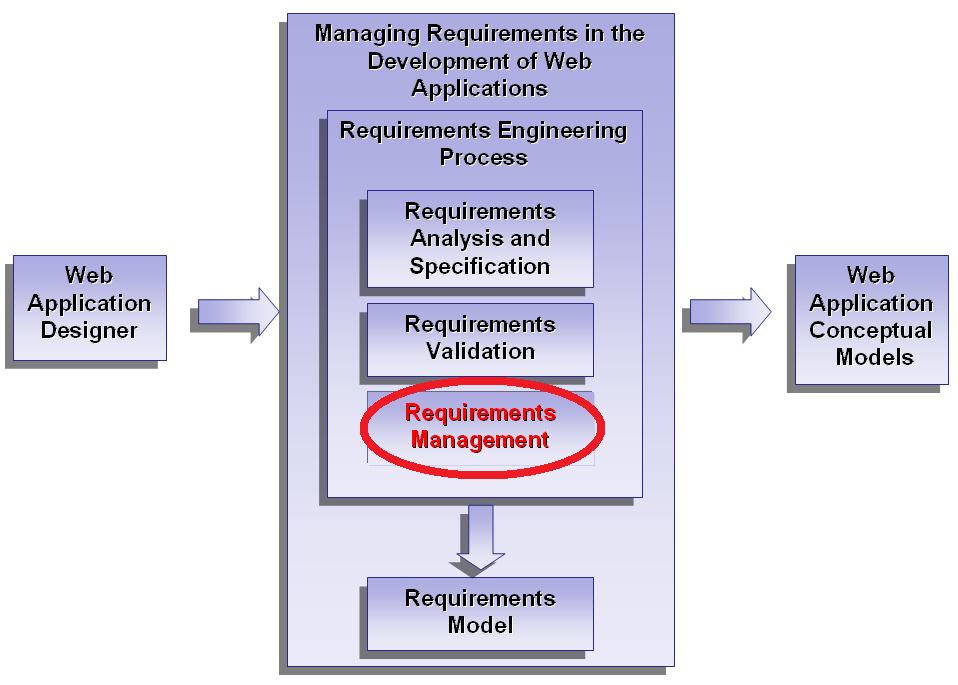
\includegraphics[width=0.7\textwidth]{img/PropuestaCap3.png}
  \end{center}
  %\caption{} \label{}
\end{figure}

En este ap�ndice, se presenta una extensi�n del Cap�tulo \ref{c5} el cual consiste en un algoritmo para manejar las dependencias entre los requisitos funcionales y los requisitos no-funcionales de la aplicaci�n Web en un contexto orientado a objetivos (\emph{goal-oriented}). Con el algoritmo, es posible comprender cu�l es el impacto en los requisitos procedente de un cambio en la estructura de modelos conceptuales que conforman la aplicaci�n Web, as� como saber qu� requisitos necesitan ser implementados para cumplir, en medida de lo posible, los prop�sitos establecidos en el an�lisis orientado a objetivos. En esta extensi�n se describe la implementaci�n del editor gr�fico WebREd para la especificaci�n de requisitos as� como la implementaci�n del algoritmo para analizar el impacto en los requisitos derivado de un cambio en los modelos conceptuales de la aplicaci�n Web.

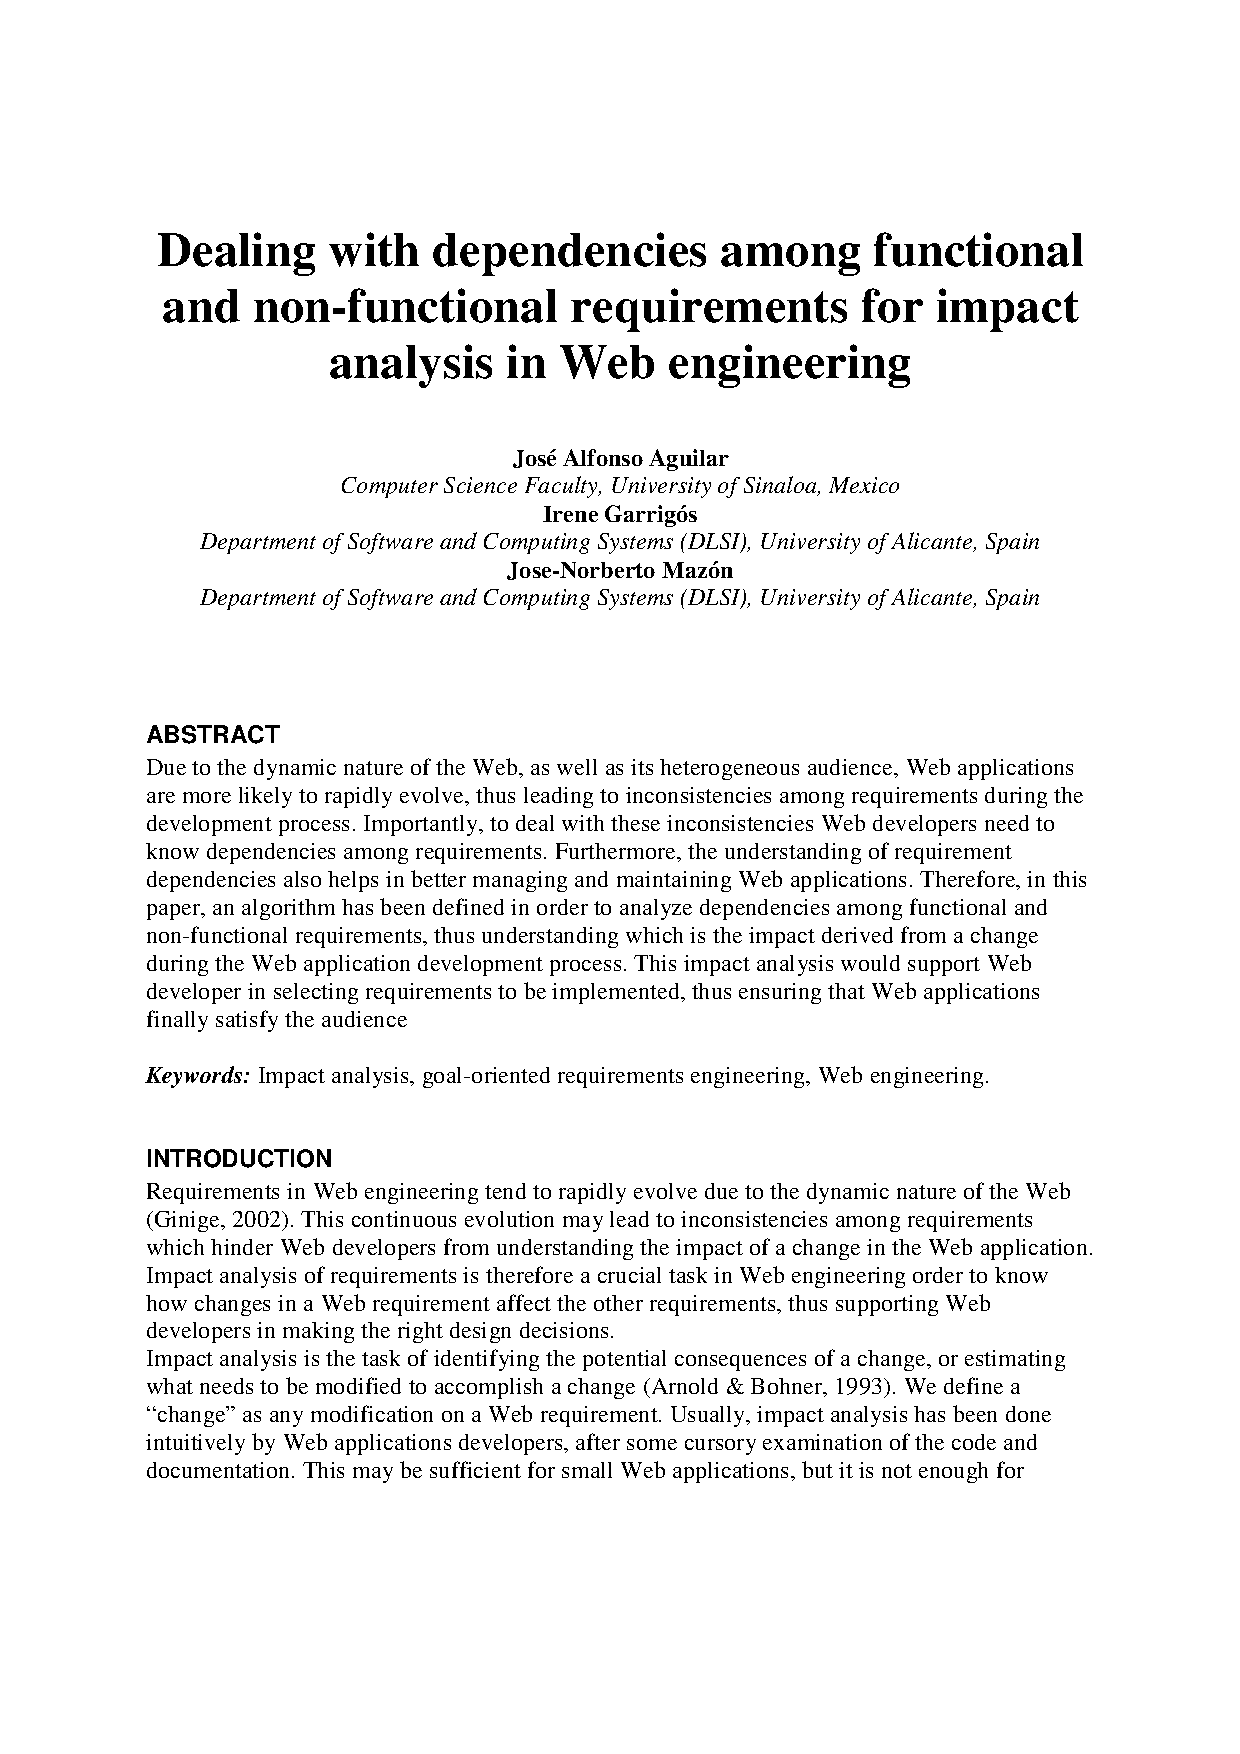
\includepdf[openright=true,pages={1-25}]{papers/apendice/aguilar_ijossp2011_CR.pdf}

